\begin{figure}
\centering
\begin{tikzpicture}
  \node (circ) {
    \begin{tikzpicture}
      \node[inner sep=0pt] (circuit) {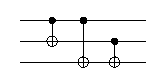
\includegraphics[scale=2]{Figures/circuits/bothEndsSimple}};  
      \node[above left=4.5mm and -7mm of circuit.west, opacity=0.9] {\footnotesize \(A\)};
      \node[left=-7mm of circuit.west, opacity=0.9] {\footnotesize \(B\)};
      \node[below left=4.5mm and -7mm of circuit.west, opacity=0.9] {\footnotesize \(C\)};
      \node[above right=0.8mm and 12.8mm of circuit.west, opacity=0.9] {\footnotesize \(\gamma\)};
      \node[below right=0.8mm and 23.6mm of circuit.west, opacity=0.9] {\footnotesize \(\beta\)};
      \node[below right=0.8mm and 34.4mm of circuit.west, opacity=0.9] {\footnotesize \(\alpha\)};
      \node[right=-3mm of circuit.north west, font=\itshape] (text) {a)};
    \end{tikzpicture}
  };
  \node[above right=-27mm and 5mm of circ] (controlHyp) {
    \begin{tikzpicture}
      \coordinate (O) at (0,0);
      \coordinate (A) at (90:10mm);
      \coordinate (B) at (210:10mm);
      \coordinate (C) at (330:10mm);
      \draw (O) -- (A);
      \draw (O) -- (B);
      \draw (O) -- (C);
      \draw (B) -- (C);
      \node[circle, right=-2.5mm of A, fill=white, inner sep=0pt, minimum size=5mm] {\(A\)};
      \node[circle, right=-2.5mm of B, fill=white, inner sep=0pt, minimum size=5mm] {\(B\)};
      \node[circle, right=-2.5mm of C, fill=white, inner sep=0pt, minimum size=5mm] {\(C\)};
      \node[above left=0mm and 13mm of A, font=\itshape] (text) {b)};
    \end{tikzpicture}
  };
  \node[right=-27mm and 15mm of circ] (targetHyp) {
    \begin{tikzpicture}
      \coordinate (O) at (0,0);
      \coordinate (A) at (90:10mm);
      \coordinate (B) at (210:10mm);
      \coordinate (C) at (330:10mm);
      \draw[ultra thick] (O) -- (A);
      \draw[ultra thick] (O) -- (B);
      \draw[ultra thick] (O) -- (C);
      \draw[ultra thick] (A) -- (B);
      \node[circle, right=-2.5mm of A, fill=white, inner sep=0pt, minimum size=5mm] {\(A\)};
      \node[circle, right=-2.5mm of B, fill=white, inner sep=0pt, minimum size=5mm] {\(B\)};
      \node[circle, right=-2.5mm of C, fill=white, inner sep=0pt, minimum size=5mm] {\(C\)};
      \node[above left=0mm and 13mm of A, font=\itshape] (text) {c)};
    \end{tikzpicture}
  };
  \node[below right=0mm and 0mm of circ] (bothHyp) {
    \begin{tikzpicture}
      \coordinate (O) at (0,0);
      \coordinate (auxC) at (4mm,3mm);
      \coordinate (auxT) at (-4mm,3mm);
      \coordinate (A) at (90:20mm);
      \coordinate (B) at (210:20mm);
      \coordinate (C) at (330:20mm);
      \draw[ultra thick] (auxT) -- (A);
      \draw[ultra thick] (auxT) -- (B);
      \draw[ultra thick] (auxT) -- (C);
      \draw[ultra thick] (A) -- (B);
      \draw (auxC) -- (A);
      \draw (auxC) -- (B);
      \draw (auxC) -- (C);
      \draw (B) -- (C);
      \node[circle, right=-2.5mm of A, fill=white, inner sep=0pt, minimum size=5mm] {\(A\)};
      \node[circle, right=-2.5mm of B, fill=white, inner sep=0pt, minimum size=5mm] {\(B\)};
      \node[circle, right=-2.5mm of C, fill=white, inner sep=0pt, minimum size=5mm] {\(C\)};
      \node[above left=0mm and 13mm of A, font=\itshape] (text) {c)};
    \end{tikzpicture}
  };
  \node[right=5mm of bothHyp] (hypergraph) {
    \begin{tikzpicture}
      \coordinate (O) at (0,0);
      \coordinate (auxA) at (90:9mm);
      \coordinate (auxC) at (330:9mm);
      \coordinate (A) at (90:18mm);
      \coordinate (B) at (210:18mm);
      \coordinate (C) at (330:18mm);
      \coordinate (a) at (270:9mm);
      \coordinate (b) at (30:9mm);
      \coordinate (c) at (150:9mm);
      \draw (auxA) -- (A);
      \draw (auxA) -- (b);
      \draw (auxA) -- (c);
      \draw[ultra thick] (auxC) -- (C);
      \draw[ultra thick] (auxC) -- (b);
      \draw[ultra thick] (auxC) -- (a);
      \draw (B) -- (a);
      \draw[ultra thick] (B) -- (c);
      \node[circle, right=-2.5mm of A, fill=white, inner sep=0pt, minimum size=5mm] {\(A\)};
      \node[circle, right=-2.5mm of B, fill=white, inner sep=0pt, minimum size=5mm] {\(B\)};
      \node[circle, right=-2.5mm of C, fill=white, inner sep=0pt, minimum size=5mm] {\(C\)};
      \node[circle, right=-2.5mm of a, fill=white, inner sep=0pt, minimum size=5mm] {\(\alpha\)};
      \node[circle, right=-2.5mm of b, fill=white, inner sep=0pt, minimum size=5mm] {\(\beta\)};
      \node[circle, right=-2.5mm of c, fill=white, inner sep=0pt, minimum size=5mm] {\(\gamma\)};
      \node[above left=0mm and 13mm of A, font=\itshape] (text) {e)};
    \end{tikzpicture}
  };
\end{tikzpicture}
\vspace*{5mm}
\caption{}
\label{fig:BothEndsChallenge}
\end{figure}

\textbf{TODO}: If the partition is \(\{\{A\},\{B,C\}\}\), then \(\alpha\) is a local CNOT, while \(\beta\) and \(\gamma\) are implemented using the common-control method. We know the common-control method must be used because the hyperedge cut is of the control type or, equivalently, because both \(\beta\) and \(\gamma\) vertices are assigned to the same block as their targets \(C\) and \(B\). Different line format for the hyperedges whether control or target.

\textbf{TODO}: Show cut that is best for common-target

\textbf{TODO}: Figure of hypergraphs from prev Fig; with control hyps, target hyps, naively. The dashed lines represent two hypothetical ways of partitioning the hypergraph. Different line format for the hyperedges whether control or target (fig:BothEndsChallenge)